\documentclass{beamer}

\mode<presentation>
{
%  \usetheme[hideothersubsections]{PaloAlto}
  \usetheme{default}
  \setbeamercovered{transparent}
}

\usepackage[english]{babel}
\usepackage[latin1]{inputenc}

\usepackage{amsmath,amssymb}
\usepackage{times} 
\usepackage[T1]{fontenc}
\usepackage{tikz}
\usepackage{pgfplots}
\usepackage{graphicx}

\usetikzlibrary{calc}

%\newrgbcolor{blue}{0 0 1}
%\newrgbcolor{red}{1 0 0}

\newcommand{\bbR}{\mathbb{R}}
\newcommand{\bbC}{\mathbb{C}}
\newcommand{\bfC}{\mathbf{C}}
\newcommand{\sfC}{\mathsf{C}}
\newcommand{\sfI}{\mathsf{I}}
\newcommand{\bfsigma}{\mathbf{\sigma}}
\newcommand{\rank}{\mathrm{rank}}
\newcommand{\orth}{\mathrm{orth}}
\newcommand{\supp}{\mathrm{supp}}
\newcommand{\tr}{\mathrm{tr}}
\newcommand{\diag}{\mathrm{diag}}
\newcommand{\calF}{\mathcal{F}}
\newcommand{\calG}{\mathcal{G}}
\newcommand{\lambdamin}{\lambda_{\mathrm{min}}}
\newcommand{\lambdamax}{\lambda_{\mathrm{max}}}
\newcommand{\sigmamin}{\sigma_{\mathrm{min}}}
\newcommand{\sigmamax}{\sigma_{\mathrm{max}}}

\title[CS 5220, Spring 2014]{Lecture 2: Useful Tools and Cluster Warm-up
(An Interactive Tutorial)}
\author[]{Nicolas Savva}
\date[]{28 Jan 2014}


\begin{document}

\begin{frame}
  \titlepage
\end{frame}

\begin{frame}
  \frametitle{Disclaimer}

  \begin{itemize}
  \item Quick overview
    \begin{itemize}
    \item nothing new for some...
    \item overwhelming for others
    \end{itemize}
  \item Similar information available on class wiki
  \item Be able to do HW0 with ease after today
  \item Please ask questions
  \end{itemize}
\end{frame}

\begin{frame}
  \frametitle{Logistics}

  \begin{itemize}
  \item Everybody in the class should be on CMS by now
  \url{http://cms.csuglab.cornell.edu/web/guest}
  \item The enrollment cap has been increased to the room limit
(several seats are available)
  \item If you cannot see the course under CMS or log in to the cluster please email us with your netID
  \item HW0 is out (due Tuesday Feb 4th)
  \end{itemize}
\end{frame}

\begin{frame}
  \frametitle{Today}

  \begin{itemize}
  \item Connecting to the cluster
  \item Basic usage of the shell
  \item Version control
  \item Running and monitoring cluster jobs
  \item HW0 walkthrough 
  \item More demos (if time permits)
  \end{itemize}
\end{frame}

\begin{frame}
  \frametitle{C4 cluster}

  \begin{itemize}
  \item Rocks linux cluster (V6.1)
  \url{http://www.rocksclusters.org/wordpress/}\\
  \t Heterogeneous nodes
  \item HTCondor scheduler (v7.8.5)\\
  \url{http://research.cs.wisc.edu/htcondor/}\\ 
  use to submit and monitor jobs on cluster
  \item Ganglia activity monitor
  \url{http://c4.coecis.cornell.edu/ganglia/}
  \end{itemize}
\end{frame}

\begin{frame}
  \frametitle{C4 cluster machines}
  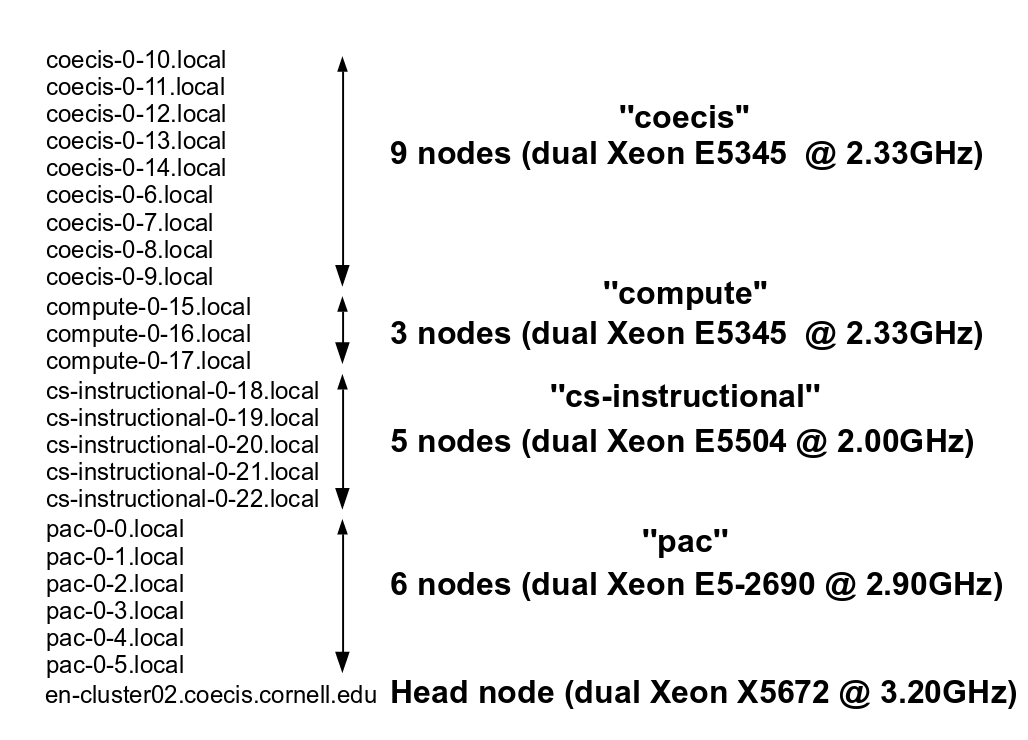
\includegraphics[width=1\textwidth]{c4overview}
\end{frame}

\begin{frame}
  \frametitle{ssh access to cluster}

  \begin{itemize}
  \item Use a Terminal under OS X or Linux
  \item PuTTY or Cygwin for windows
  \item Authenticate with Cornell NetID and password \\
  %\begin{center}
  \it{ssh netID@c4.coecis.cornell.edu}
  %\end{center}
  \end{itemize}
\end{frame}

\begin{frame}
  \frametitle{Terminal prompt}

  \begin{itemize}
  \item Type the following for a one-off initialization: \\
  \vspace{5mm}
  \it{/share/cs-instructional/cs5220/script/setup.sh} \\
  \vspace{5mm}
  This appends commands to .bashrc and .bash\_profile to \\
  automatically set a class-related environment every time \\
  you log in.
  \end{itemize}
\end{frame}

\begin{frame}
  \frametitle{Customize the prompt}

  Google customize \$PS1 \\
  add your version to the .bashrc file\\
  \vspace{5mm}
  \it{export \$PS1 = ...}
  \vspace{10mm}

  \textbackslash u		username\\
  \textbackslash h		hostname\\
  \it{pwd} 	working directory path\\
  \textbackslash n 		new line\\

\end{frame}

\begin{frame}
  \frametitle{Some bash commands}
  \begin{center}
    \begin{tabular}{ c c c c }
    ls & w & chmod & ssh \\
    cd & ps & export & scp \\
    pwd & jobs & set & tar \\
    mkdir & fg & alias & vi \\
    rmdir & bg & exit & nano \\
    mv & kill & history & which \\
    cp & Ctrl + C & | & man \\
    grep &  Ctrl + Z & find & echo \\
    \end{tabular}
  . .. > >> < << \&
  \end{center}
  \vspace{5mm}  

  If you are not particularly familiar with the above please \\
  check out the following tutorial :
  \url{http://software-carpentry.org/v4/shell/ }
\end{frame}

\begin{frame}
  \frametitle{For more details}
  \begin{itemize}
  \item \it{The UNIX programming environment} \\
  by Kernighan \& Pike \\
  \url{http://cornell.worldcat.org/title/unix-programming-environment/} \\
  \item \it{Learning the bash shell} \\
  by Newham \& Rosenblatt \\
  \url{http://cornell.worldcat.org/title/learning-the-bash-shell/} \\
  \end{itemize}

  \vspace{5mm}  
  Both are available through the Cornell library
\end{frame}

\begin{frame}
  \frametitle{Terminal multiplexer (tmux)}

  \begin{center}
  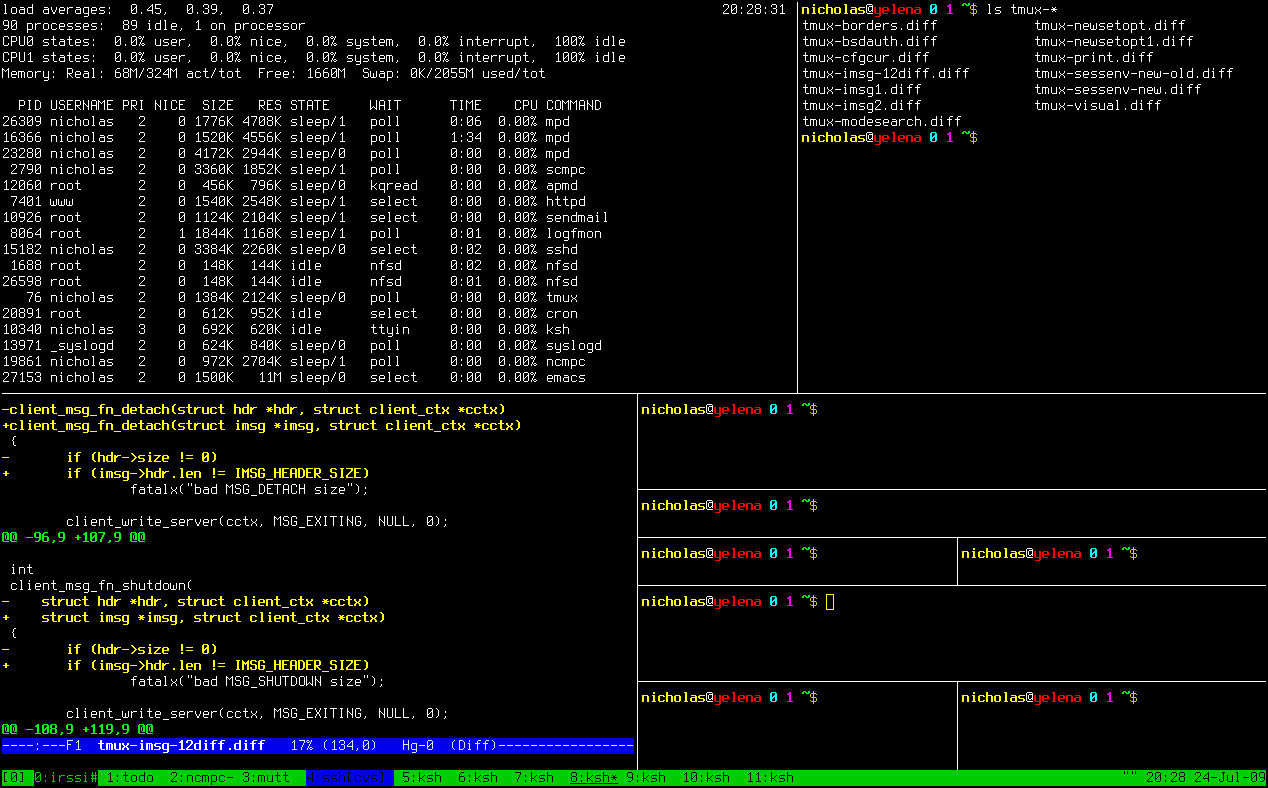
\includegraphics[width=0.8\textwidth]{tmux} \\
  \url{http://tmux.sourceforge.net/}
  \end{center}
  \begin{itemize}
  \item Concurrently view/manage multiple programs in one terminal
  \item Read documentation (key-binding / configuration)
  \item Edit .tmux.conf
  \end{itemize}

\end{frame}

\begin{frame}
  \frametitle{Version Control Systems (VCS)}

  \begin{itemize}
  \item Why version control?
  \vspace{5mm}
    \begin{itemize}
    \item Keep revision history
    \vspace{5mm}
    \item Easy way to share files between machines 
    \vspace{5mm}
    \item More effective collaboration
    \vspace{5mm}
    \item (Remote) backup
    \end{itemize}
  \end{itemize}

\end{frame}

\begin{frame}
  \frametitle{VCS - many flavors}

  \begin{itemize}
  \item Distributed
  \vspace{5mm}
    \begin{itemize}
    \item Git
    \item Mercurial (Hg) 
    \item Bazaar \\
    ...
    \end{itemize}
    \vspace{5mm}
  \item Client-server
    \begin{itemize}
    \item Subversion (SVN)
    \item CVS \\
    ...
    \end{itemize}
  \end{itemize}

\end{frame}

\begin{frame}
  \frametitle{Repositories - Host projects online}

  \begin{itemize}
  \item Bitbucket (Mercurial or Git)
  \item Github (Git)
  \item Launchpad (Bazaar)
  \item Google Code (SVN, Mercurial or Git)
  \item Microsoft CodePlex (SVN, Mercurial or Git)
  \item Sourceforge (CVS, SVN, Bazaar, Git or Mercurial)
  \item Cornell Forge (SVN) -  \url{http://forge.cornell.edu}
  \end{itemize}

\end{frame}

\begin{frame}
  \frametitle{Bitbucket}

  \begin{itemize}
  \item Class repository and wiki are hosted on Bitbucket: \\
  \url{https://bitbucket.org/dbindel/cs5220-s14/} \\
  Sign up for a free account \\
  \item Git tutorial \\
  \url{https://www.atlassian.com/git/tutorial} \\
  \item Pro Git book \\
  \url{http://git-scm.com/documentation }\\
  \item Git (Interactive) Cheat Sheet  \\
  \url{http://ndpsoftware.com/git-cheatsheet.html} \\
  \item Git commands overview
  \url{https://www.atlassian.com/dms/wac/images/landing/git/atlassian\_git\_cheatsheet.pdf}
  \end{itemize}
\end{frame}


\begin{frame}
  \frametitle{Making a local copy}

  \begin{itemize}
  \item Clone the class repository
  \vspace{5mm}
  \begin{center}
    \it{git clone https://bitbucket.org/dbindel/cs5220-s14.git}
  \end{center}
  \vspace{5mm}
  The folder cs5220-s14 now contains local copy
  \end{itemize}

\end{frame}

\begin{frame}
  \frametitle{Git basics demo}

  \begin{itemize}
  \item git clone
  \item git add
  \item git diff
  \item git commit
  \item git log
  \item git remote
  \item git pull
  \item git push
  \end{itemize}
  \vspace{5mm}
  Please look at the cheat sheet and tutorials for more functionality

\end{frame}

\begin{frame}
  \frametitle{Graphical Interfaces available}

  \begin{itemize}
  \item EGit (Git with Eclipse IDE) \\
  \url{http://www.eclipse.org/egit/} \\
  \vspace{5mm}
  \item Subclipse (SVN with Eclipse) \\
  \url{http://subclipse.tigris.org/}\\
  \vspace{5mm}
  \item SourceTree (Git and Mercurial GUI under Windows or Mac) \\
  \url{http://www.sourcetreeapp.com/} \\
  \vspace{5mm}
  \item TortoiseSVN, TortoiseHg, TortoiseGit... series (mostly Windows)
  \end{itemize}

\end{frame}

\begin{frame}
  \frametitle{Eclipse PTP (Parallel Tools Platform)}

  \begin{itemize}
  \item IDE for developing parallel applications
  \item Support MPI, OpenMP, UPC
  \item Parallel debugger
  \item Various profiling tools
  \item Some issues running on c4 cluster
  \item Experiment with it on your own machine
  \item Please don't use PTP remotely on c4 right now
  \end{itemize}

  \begin{center}
  \url{http://www.eclipse.org/ptp/}
  \end{center}

\end{frame}

\begin{frame}
  \frametitle{Using HTCondor}

  \begin{itemize}
  \item condor\_status [-claimed -avail -master -verbose]
  \item condor\_q [ -analyze -run -hold]
  \item condor\_submit 
  \item condor\_hold
  \item condo\_release
  \item condor\_rm
  \item condor\_history [ -backwards -forwards -match]
  \end{itemize}
  [ -constraint -format ]

\end{frame}

\begin{frame}
  \frametitle{HTCondor CS5220 wrapper scripts}

  \begin{itemize}
  \item csub (serial submissions)
  \vspace{5mm}
  \item mpisub (Message Passing Interface)
  \vspace{5mm}
  \item upcsub (Unified Parallel C)
  \vspace{5mm}
  \item ompsub (OpenMP: Open Multi-Processing)
  \end{itemize}
  \vspace{10mm}
  \small \url{https://bitbucket.org/dbindel/c4-pkg}
\end{frame}

\begin{frame}
  \frametitle{Environment modules}
  
  Make it easy to install:\\
  \begin{itemize}
  \item different versions of software packages\\
  \item software packages that might conflict\\
  \end{itemize}
  \vspace{5mm}
  \begin{itemize}
  \item module list
  \vspace{5mm}
  \item module avail
  \vspace{5mm}
  \item module load \\
  module add
  \vspace{5mm}
  \item module unload \\
  module rm
  \end{itemize}
  \small \url{https://bitbucket.org/dbindel/cs5220-s14/wiki/modules}
\end{frame}

\begin{frame}
  \frametitle{Homework 0 walkthrough}
  
  Steps:\\
  \vspace{5mm}
  \begin{itemize}
  \item Clone class repo
  \vspace{5mm}
  \item membench
  \vspace{5mm}
  \item membench with ClassAd requirements
  \vspace{5mm}
  \item HTCondor job management
  \vspace{5mm}
  \item pinfo
  \vspace{5mm}
  \item Retrieve the results (using sftp or scp)
  \end{itemize}
  \small \url{http://bitbucket.org/dbindel/cs5220-s14/wiki/HW0}
\end{frame}

\begin{frame}
  \frametitle{Additional Demos...}

\end{frame}

\end{document}



